\chapter{Results}
\label{chap:results}

% overview
% what do the results show

\section{Experimental Setup}

% Hardware stats AMD Ryzen 7 5800X @ 8x3.8GHz (-4.7 GHz), 128GB RAM, Ubuntu 22.04.2 LTS
% random generator seed based to recreate instances
% evaluate each options sorting with same seeds
% timeout at 600s
% always assembly of target polyominoes from initial
% list experiments


\section{Assembly for Target Size}

This experiment was conducted with randomly generated polyominoes and initial configuration of specific target sizes $n$.
To maximize the variety of possible polyomino-shapes the number of red cubes is set to $n_\textit{red} = \lfloor \frac{n}{2} \rfloor$ \cite{Lu2021}.
Because of the variety, this experiment is well-suited for not only analyzing planning time and rotational-cost, but also examine $\#\textit{local}$, $\#\textit{config}$ and $|P|$.
We worked in a quadratic workspace of size $50 r_C \times 50 r_C$ and for each target size $150$ samples where taken.

\paragraph{Time and Failure Analysis}

\begin{figure}
	\centering
	\begin{subfigure}[b]{\textwidth}
		\centering
		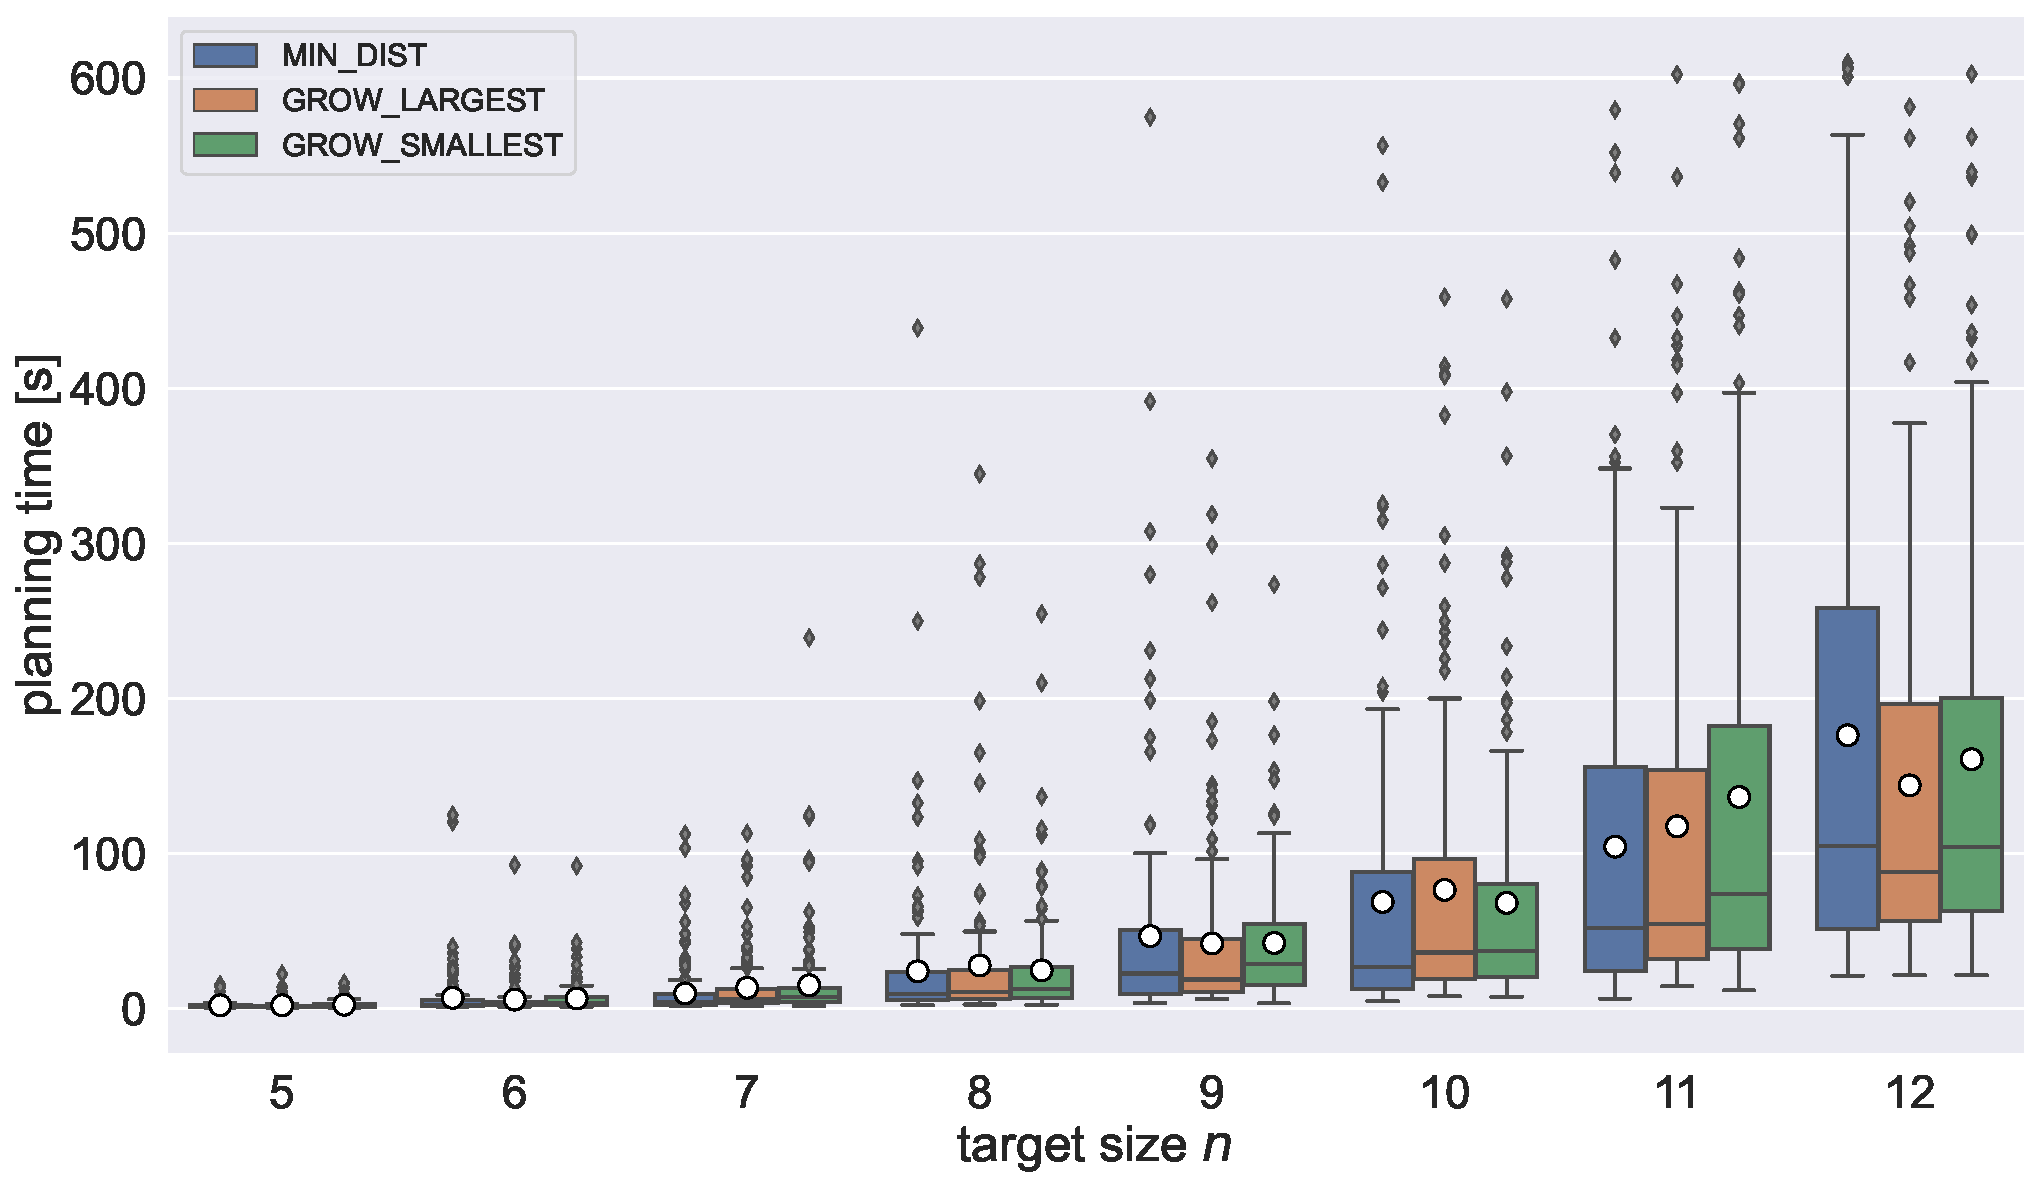
\includegraphics[width=0.9\textwidth]{figures/plots/AFN_time.pdf}
		\caption{Planning time in seconds. Only plans that did not time out are shown.}
		\label{fig:AFN_time}
	\end{subfigure}

	\begin{subfigure}[b]{\textwidth}
		\centering
		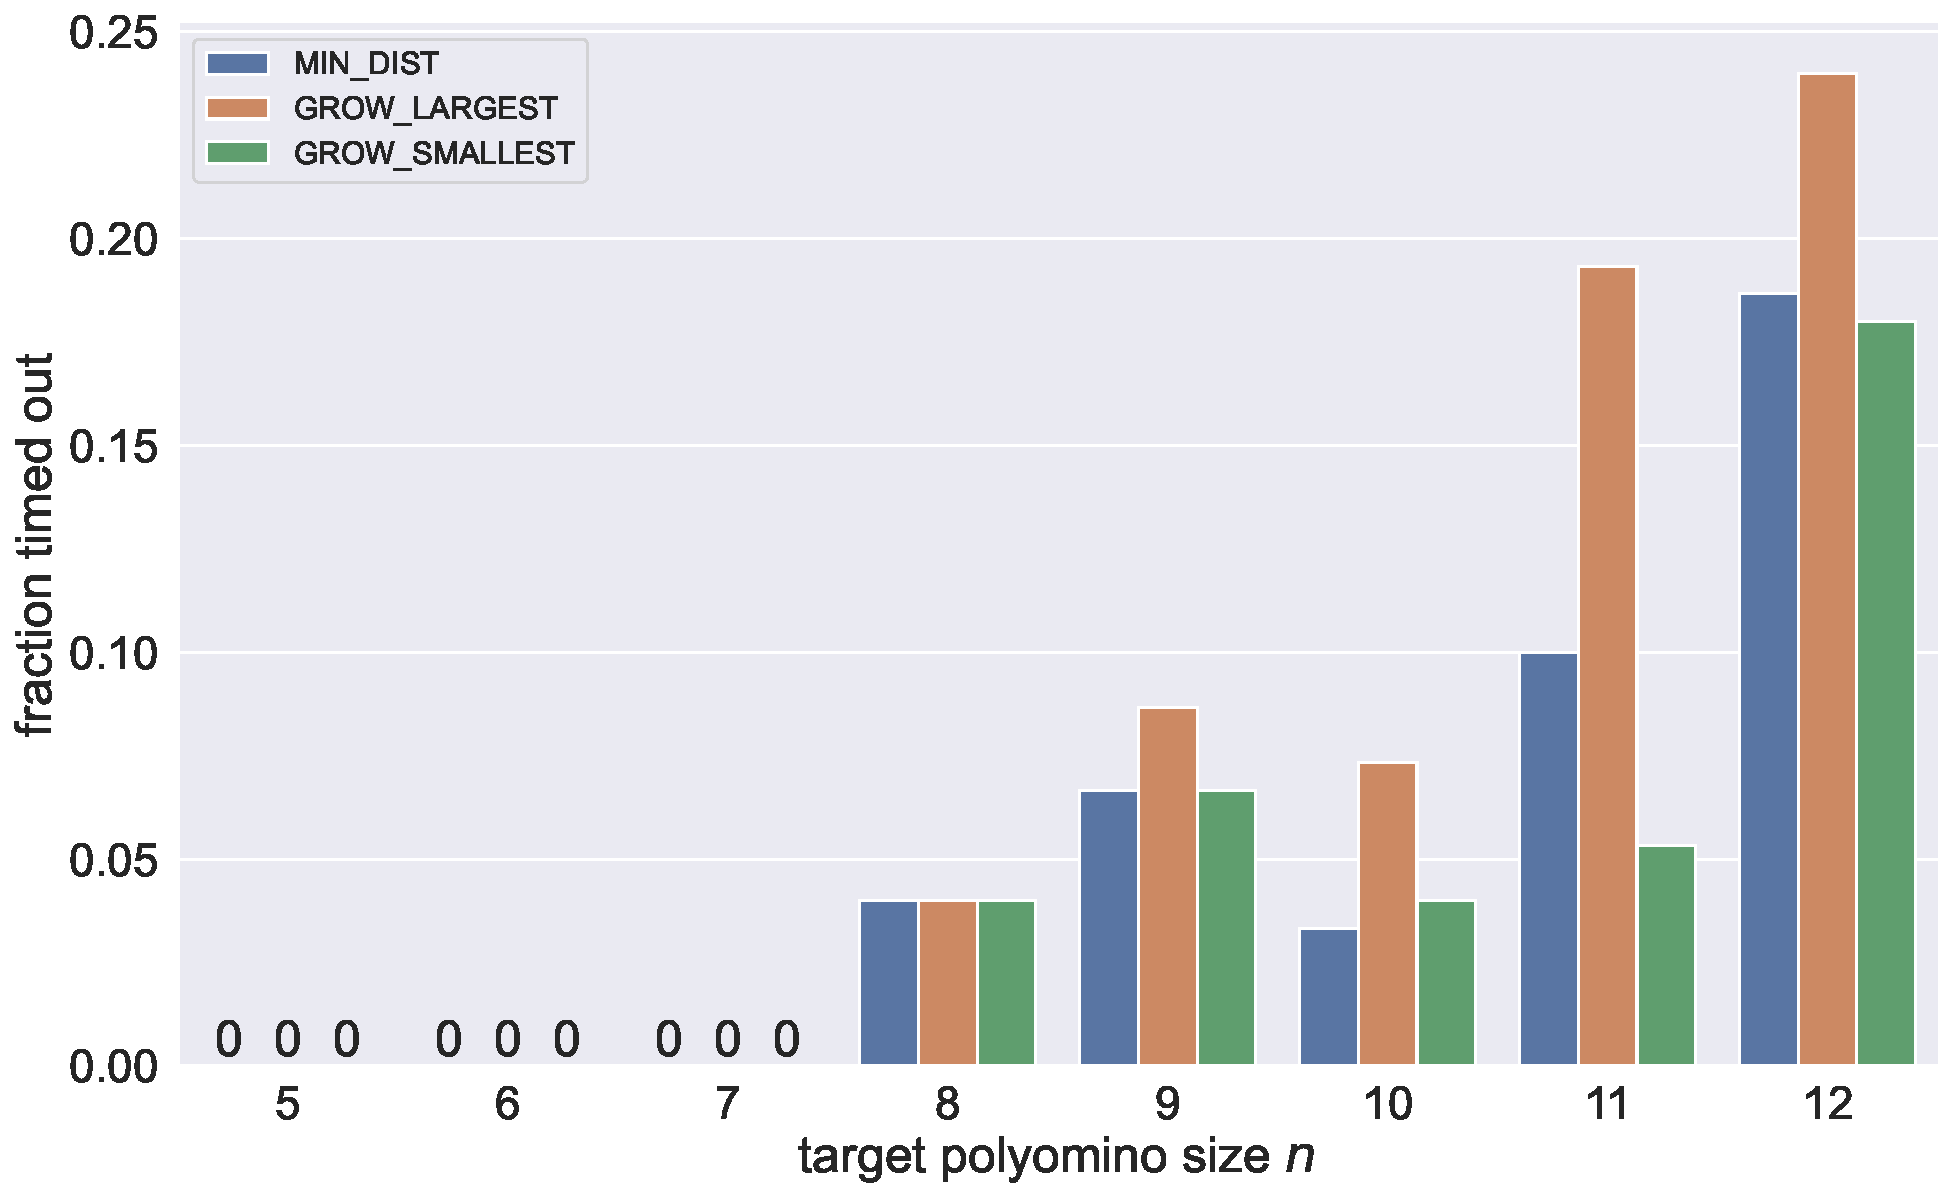
\includegraphics[width=0.9\textwidth]{figures/plots/AFN_timeout.pdf}
		\caption{Fraction of plans that timed out}
		\label{fig:AFN_timeout}
	\end{subfigure}
	\caption[Planning time and fraction timed out for different target sizes]{Planning time and fraction timed out for different target sizes $n$. All option sorting strategies are compared.}
	\label{fig:AFN_timestats}
\end{figure}



\paragraph{Cost Analysis}

\begin{figure}
	\centering
	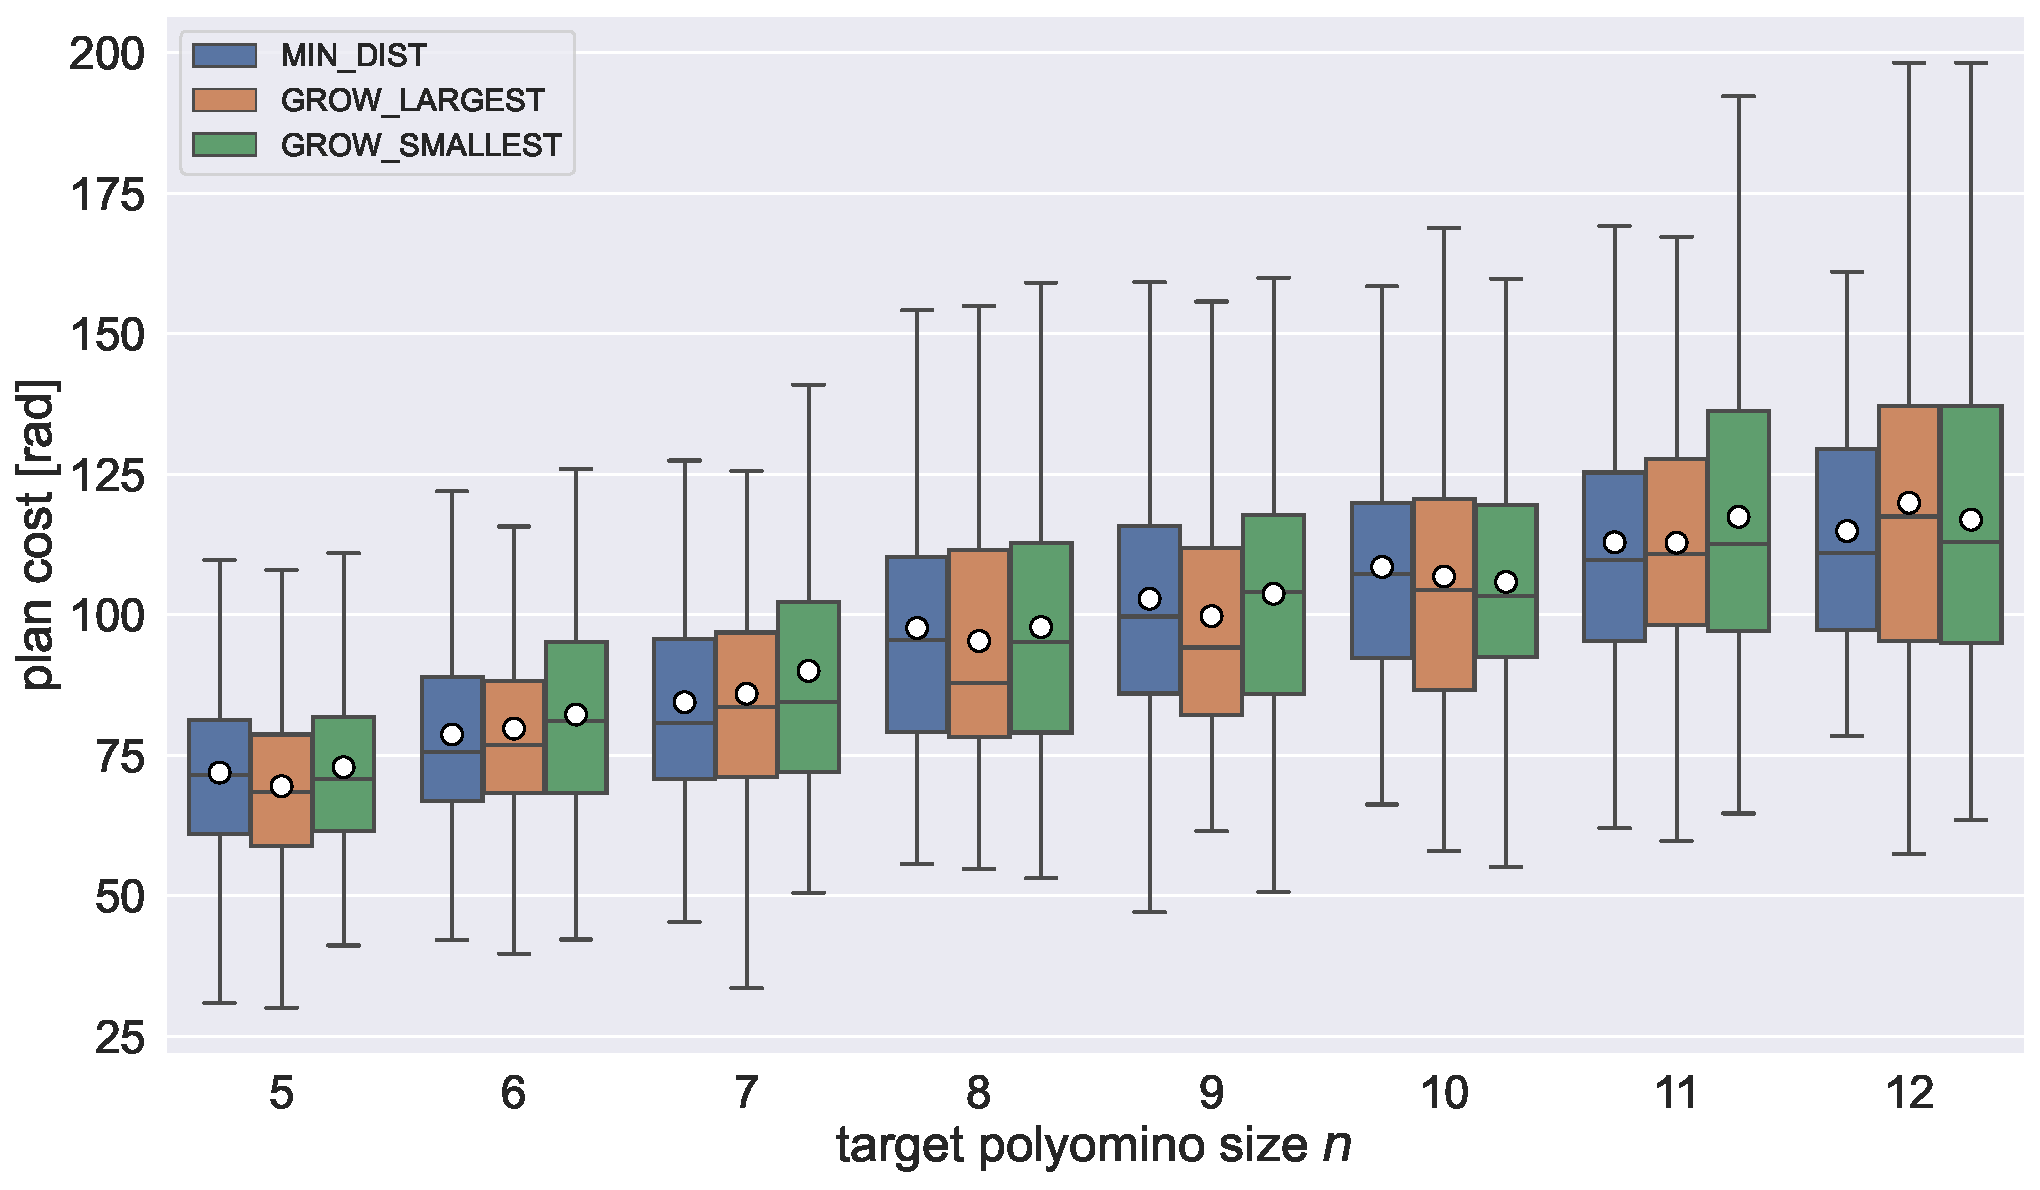
\includegraphics[width=0.9\textwidth]{figures/plots/AFN_cost.pdf}
	\caption[Plan cost for different target sizes]{Plan cost for different target sizes $n$. All option sorting strategies are compared.}
	\label{fig:AFN_cost}
\end{figure}



\paragraph{Planning Analysis}

\begin{figure}
	\centering
	\begin{subfigure}[b]{\textwidth}
		\centering
		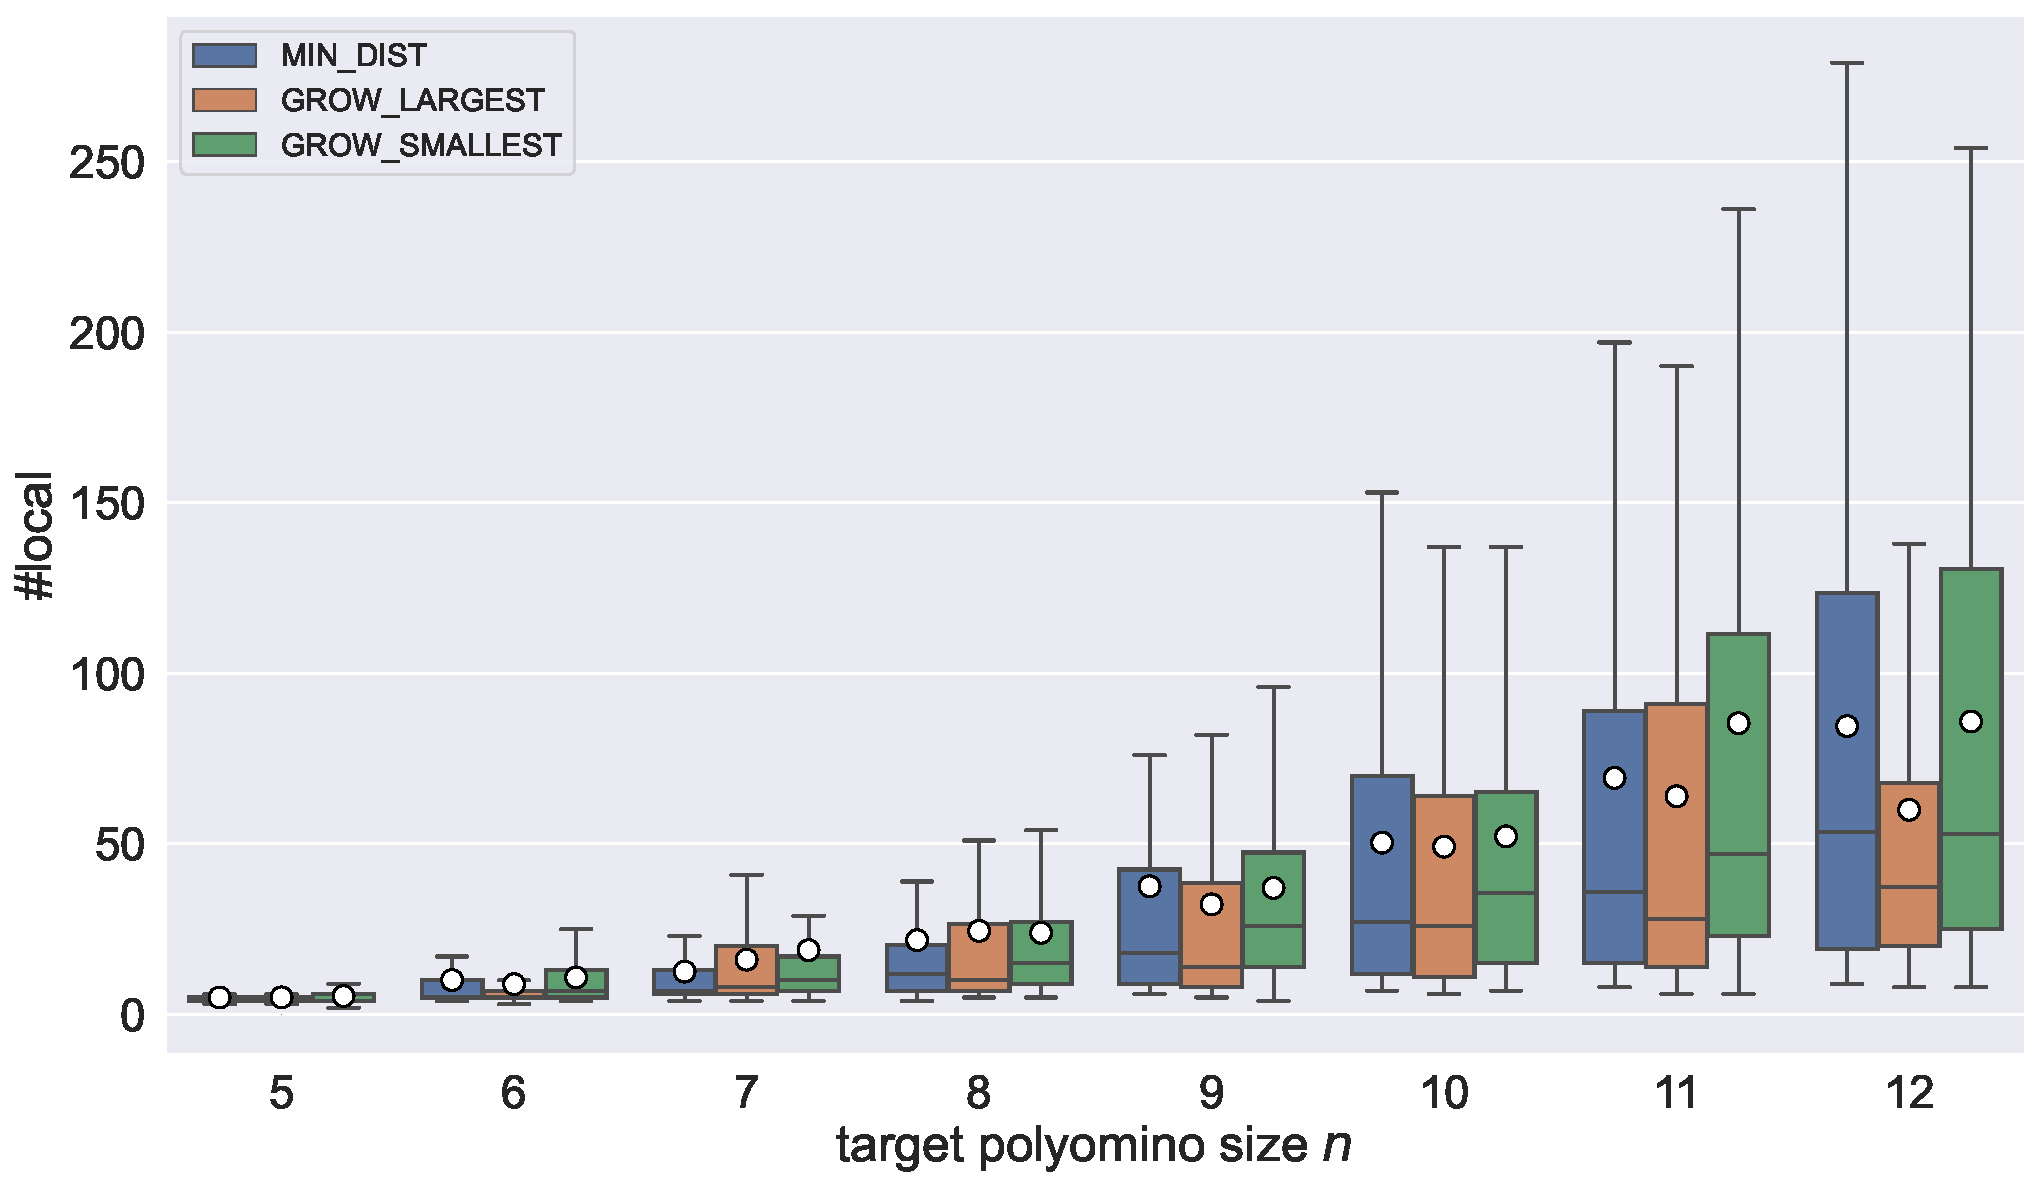
\includegraphics[width=0.9\textwidth]{figures/plots/AFN_nlocal.pdf}
		\caption{Number of simulated local plans.}
		\label{fig:AFN_nlocal}
	\end{subfigure}
	
	\begin{subfigure}[b]{\textwidth}
		\centering
		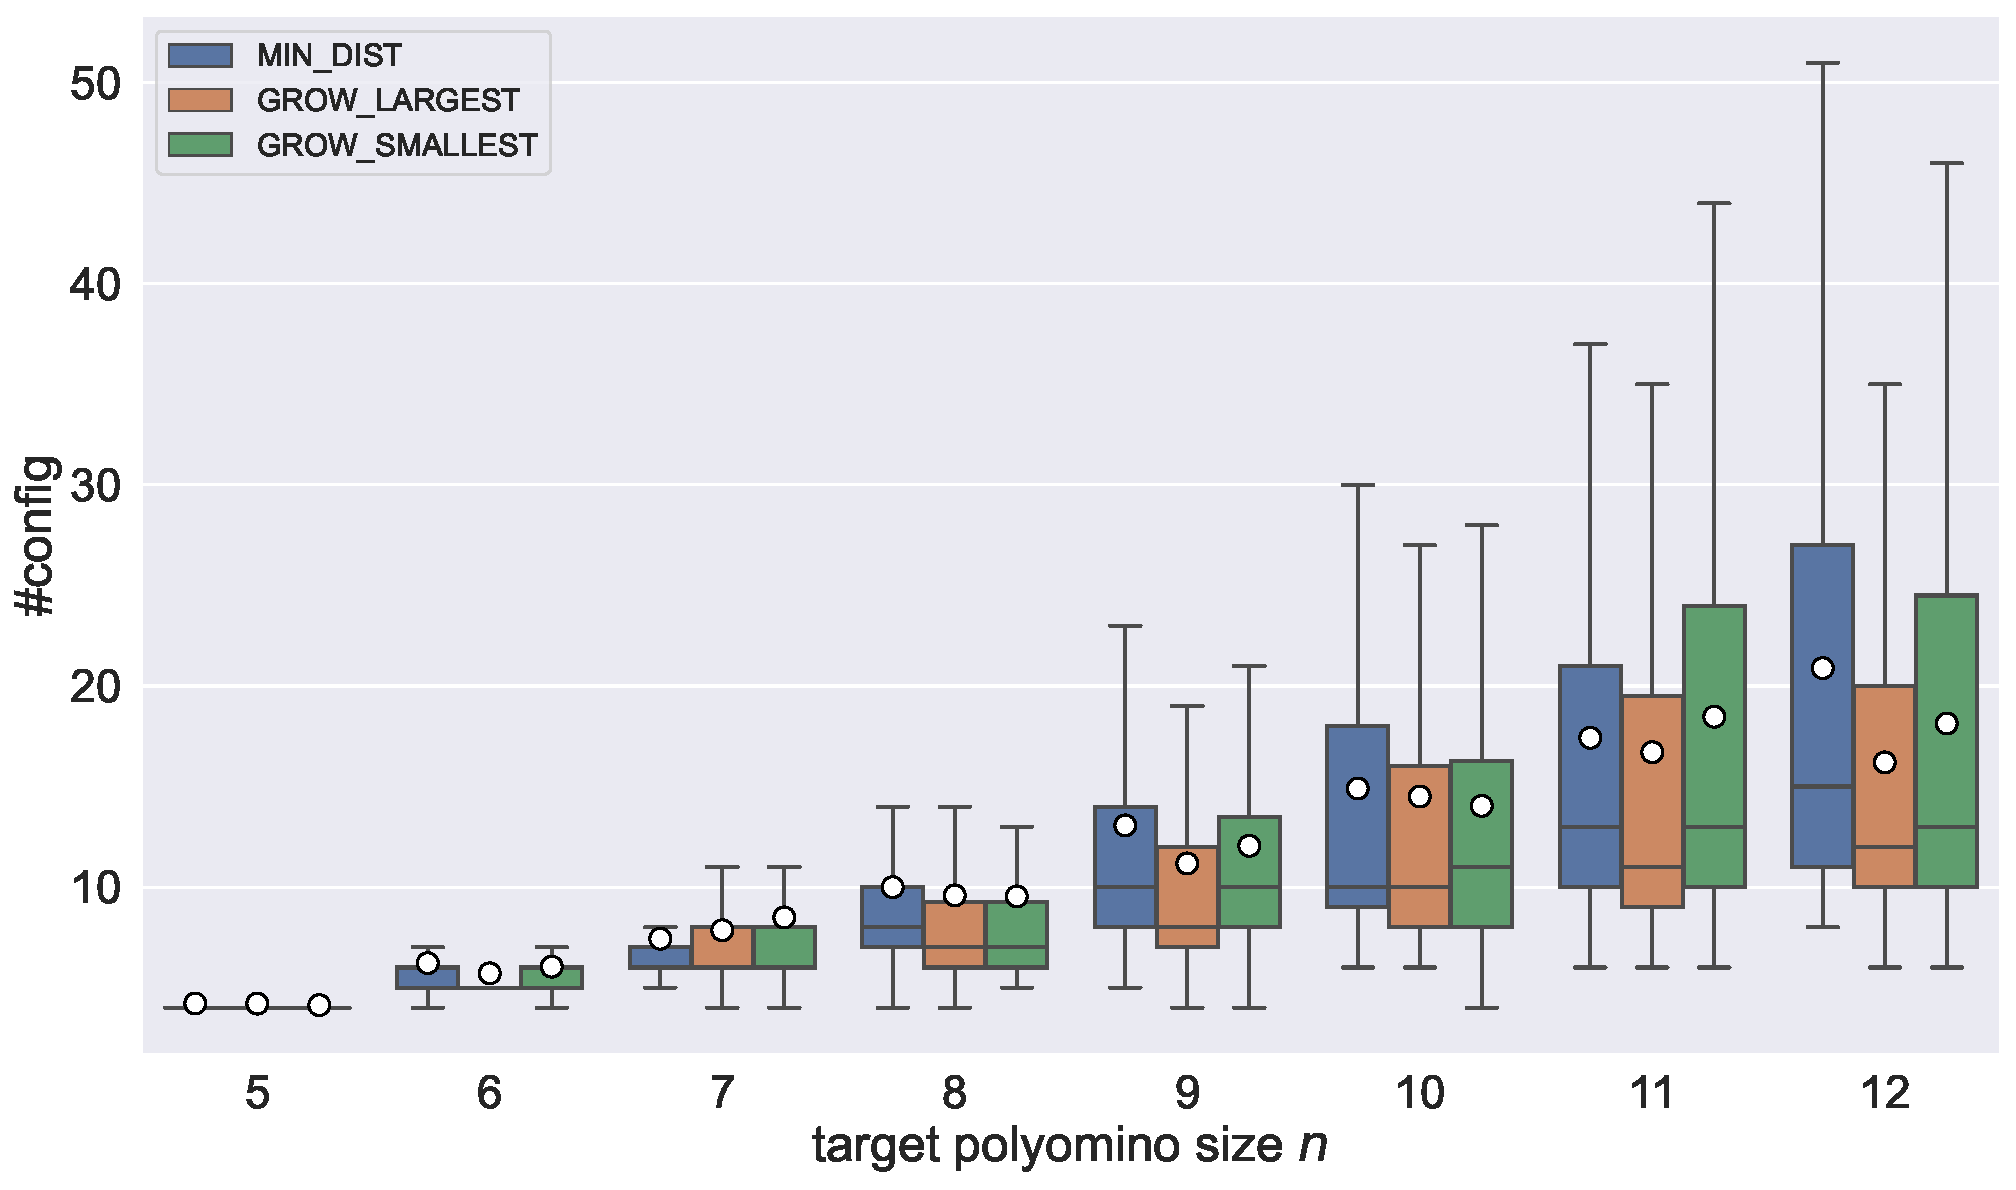
\includegraphics[width=0.9\textwidth]{figures/plots/AFN_nconfig.pdf}
		\caption{Number of explored configurations}
		\label{fig:AFN_nconfig}
	\end{subfigure}
	\caption[$\#\textit{config}$ and $\#\textit{config}$ for different target sizes]{Number of simulated local plans $\#\textit{local}$ and number of explored configurations $\#\textit{config}$ for different target sizes $n$. All option sorting strategies are compared.}
	\label{fig:AFN_planstats}
\end{figure}

\begin{figure}
	\centering
	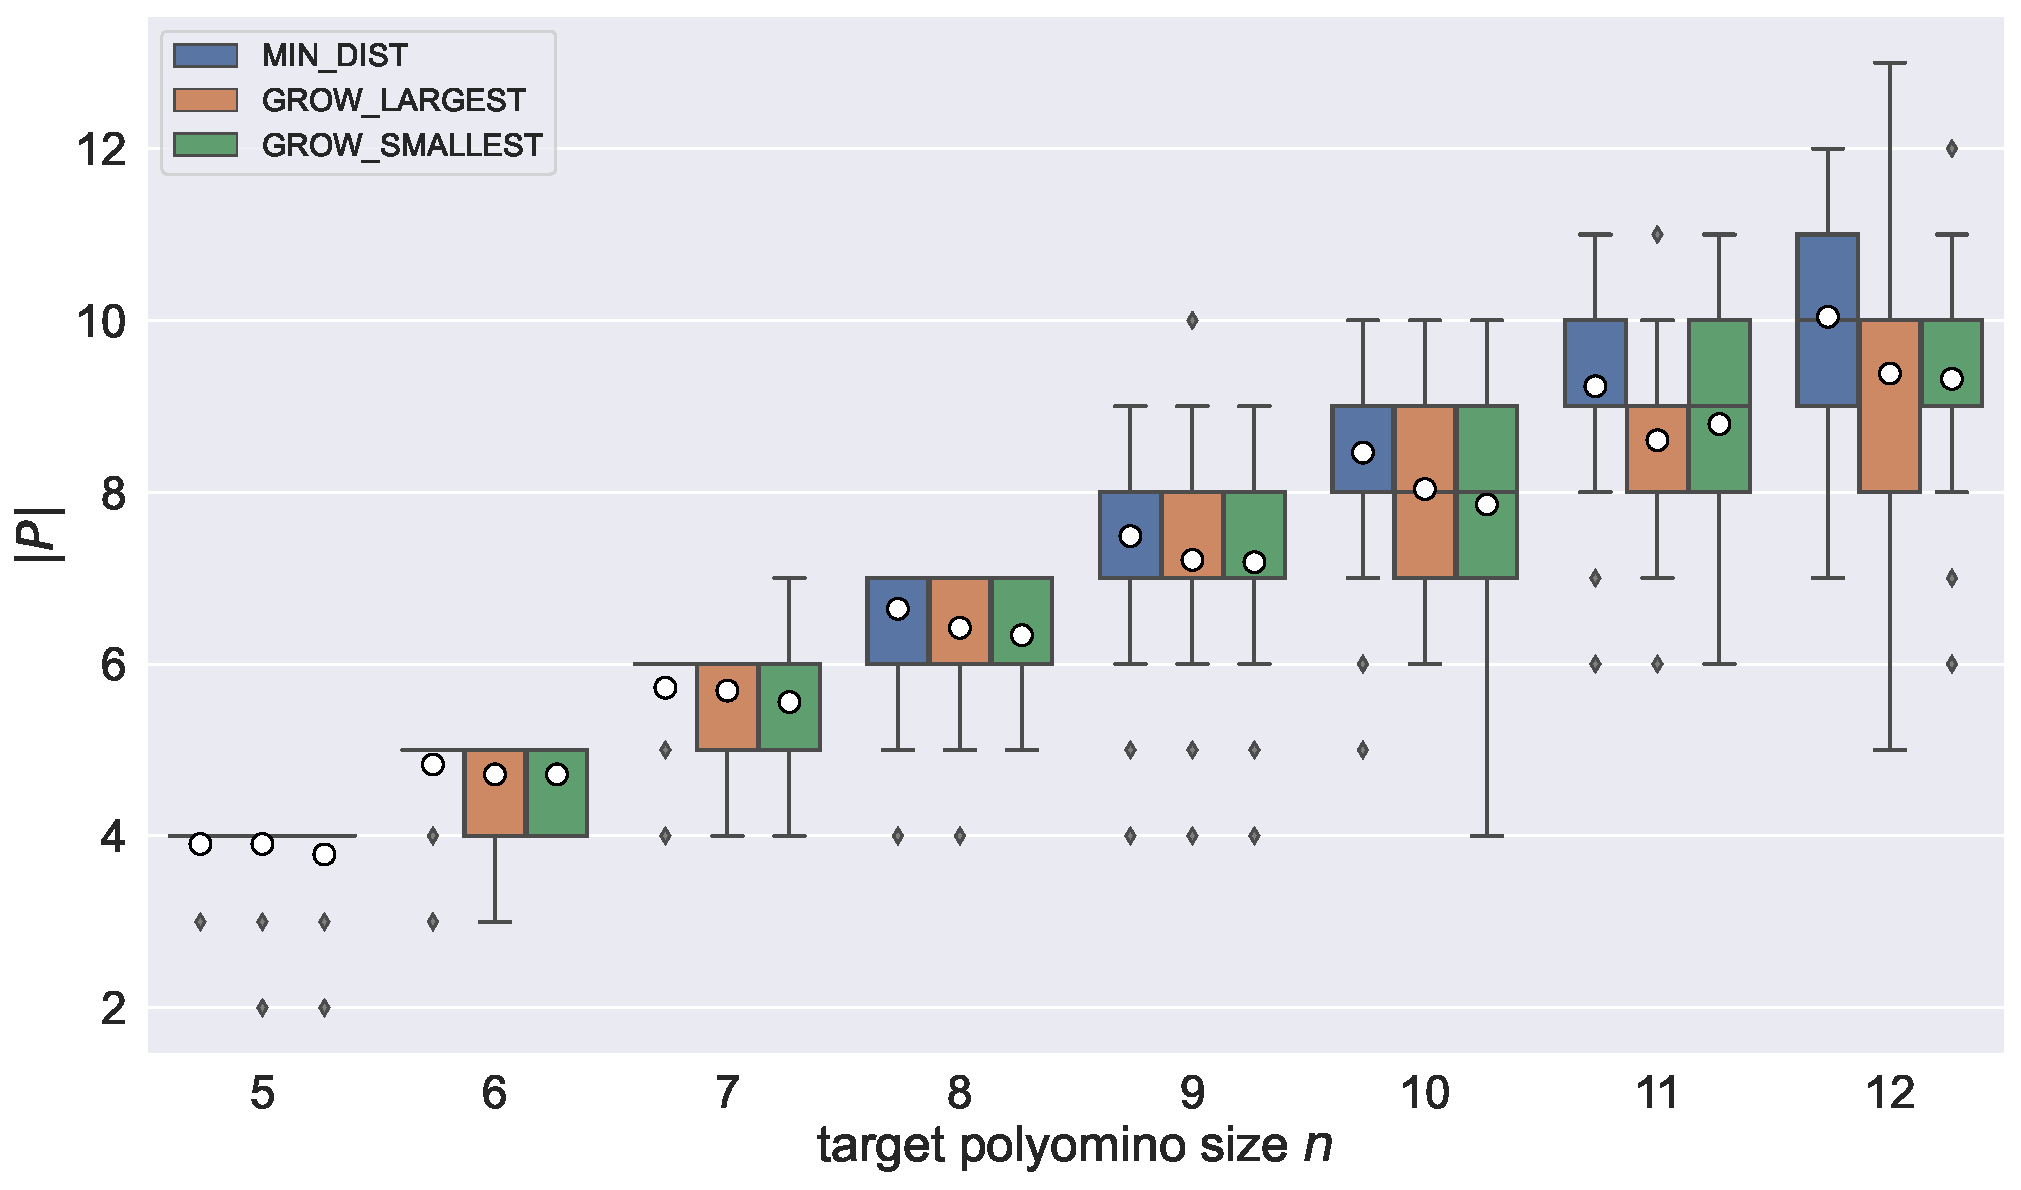
\includegraphics[width=0.9\textwidth]{figures/plots/AFN_ltg.pdf}
	\caption[Local plans in plan stack for different target sizes]{Local plans in plan stack $|P|$ for different target sizes $n$. All option sorting strategies are compared.}
	\label{fig:AFN_ltg}
\end{figure}




\section{Assembly for Target Shape}

\begin{figure}
	\centering
	\begin{subfigure}[b]{\textwidth}
		\centering
		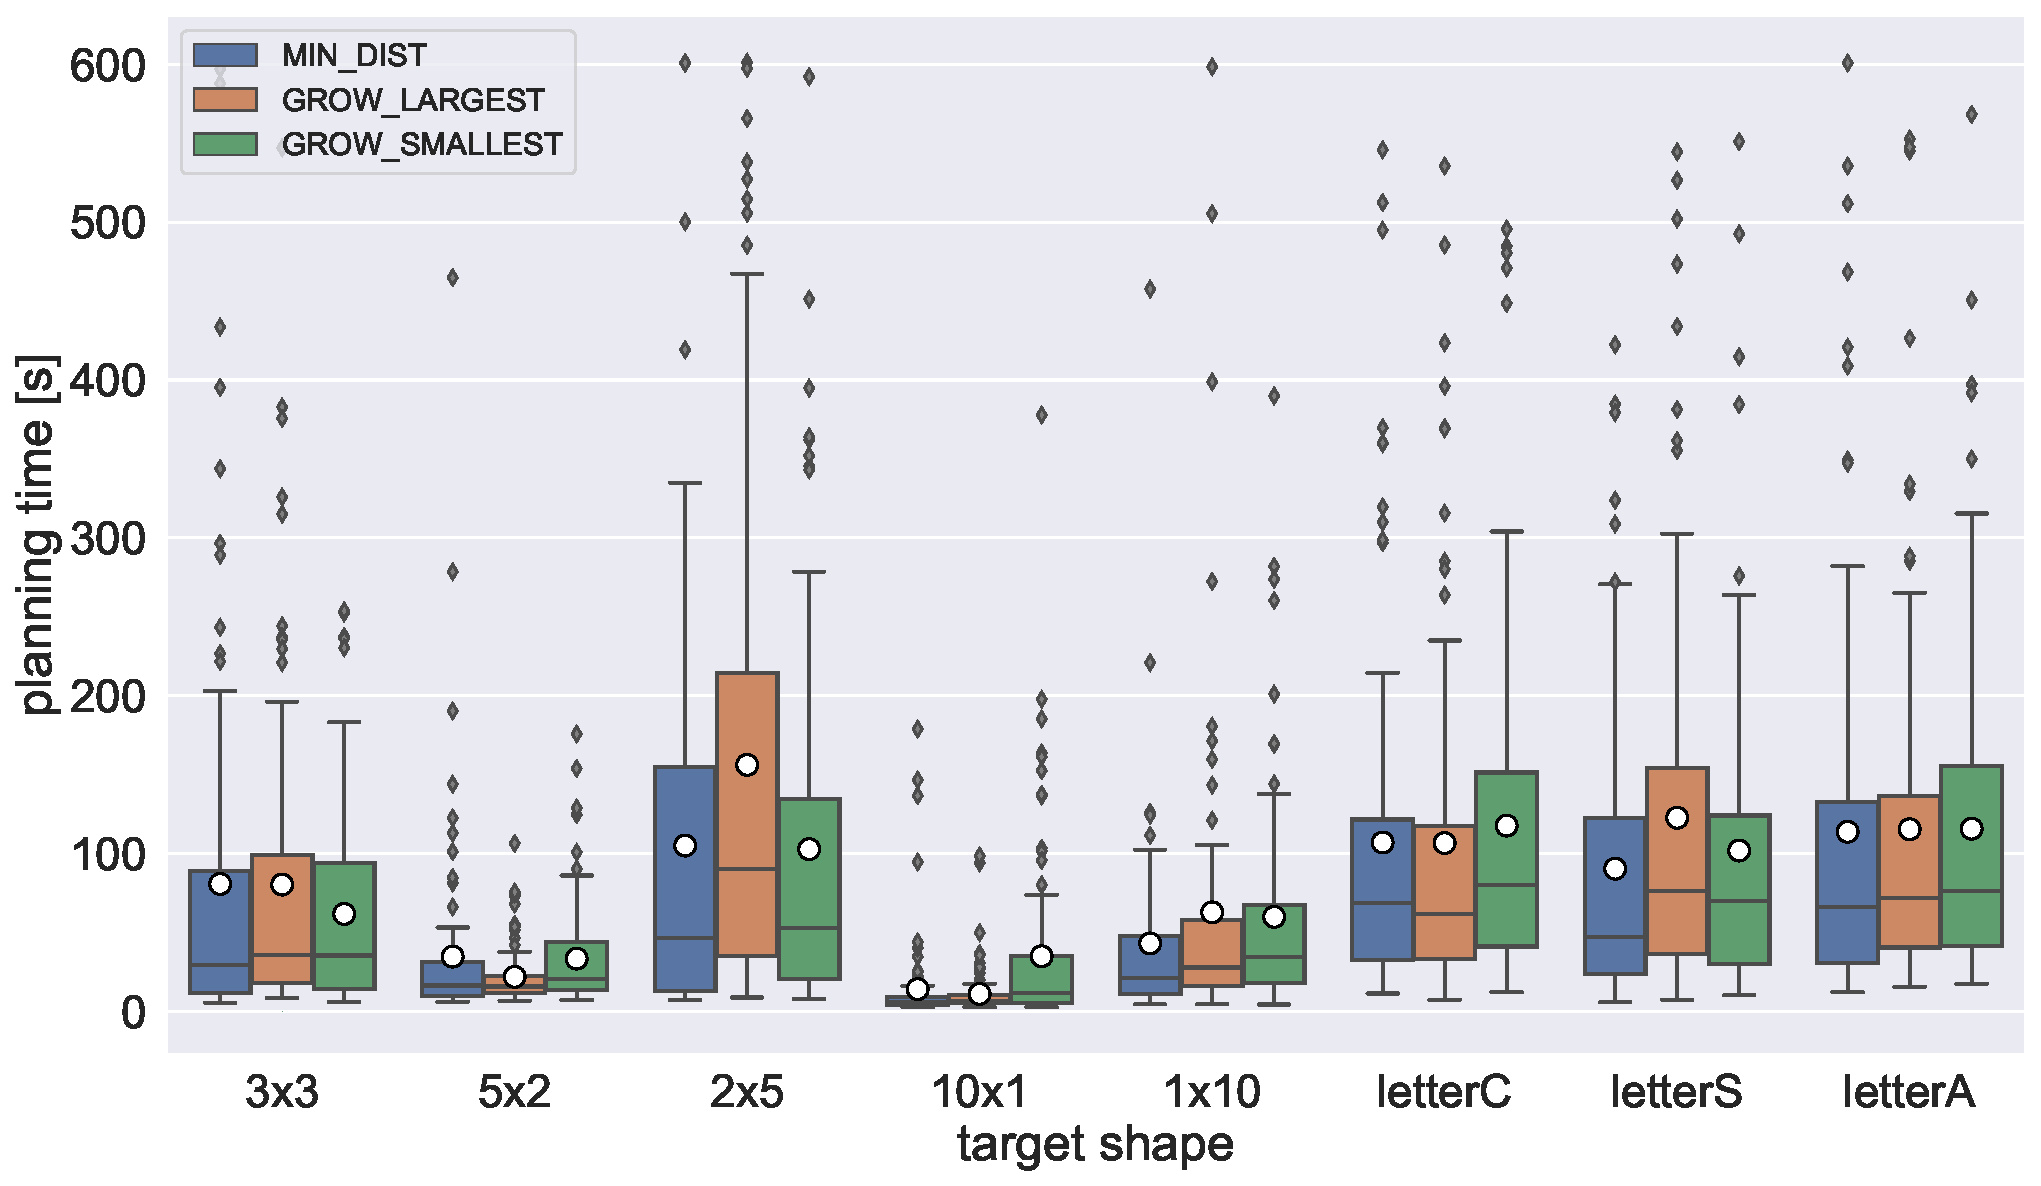
\includegraphics[width=0.9\textwidth]{figures/plots/AFTS_time.pdf}
		\caption{}
		\label{fig:AFTS_time}
	\end{subfigure}
	
	\begin{subfigure}[b]{\textwidth}
		\centering
		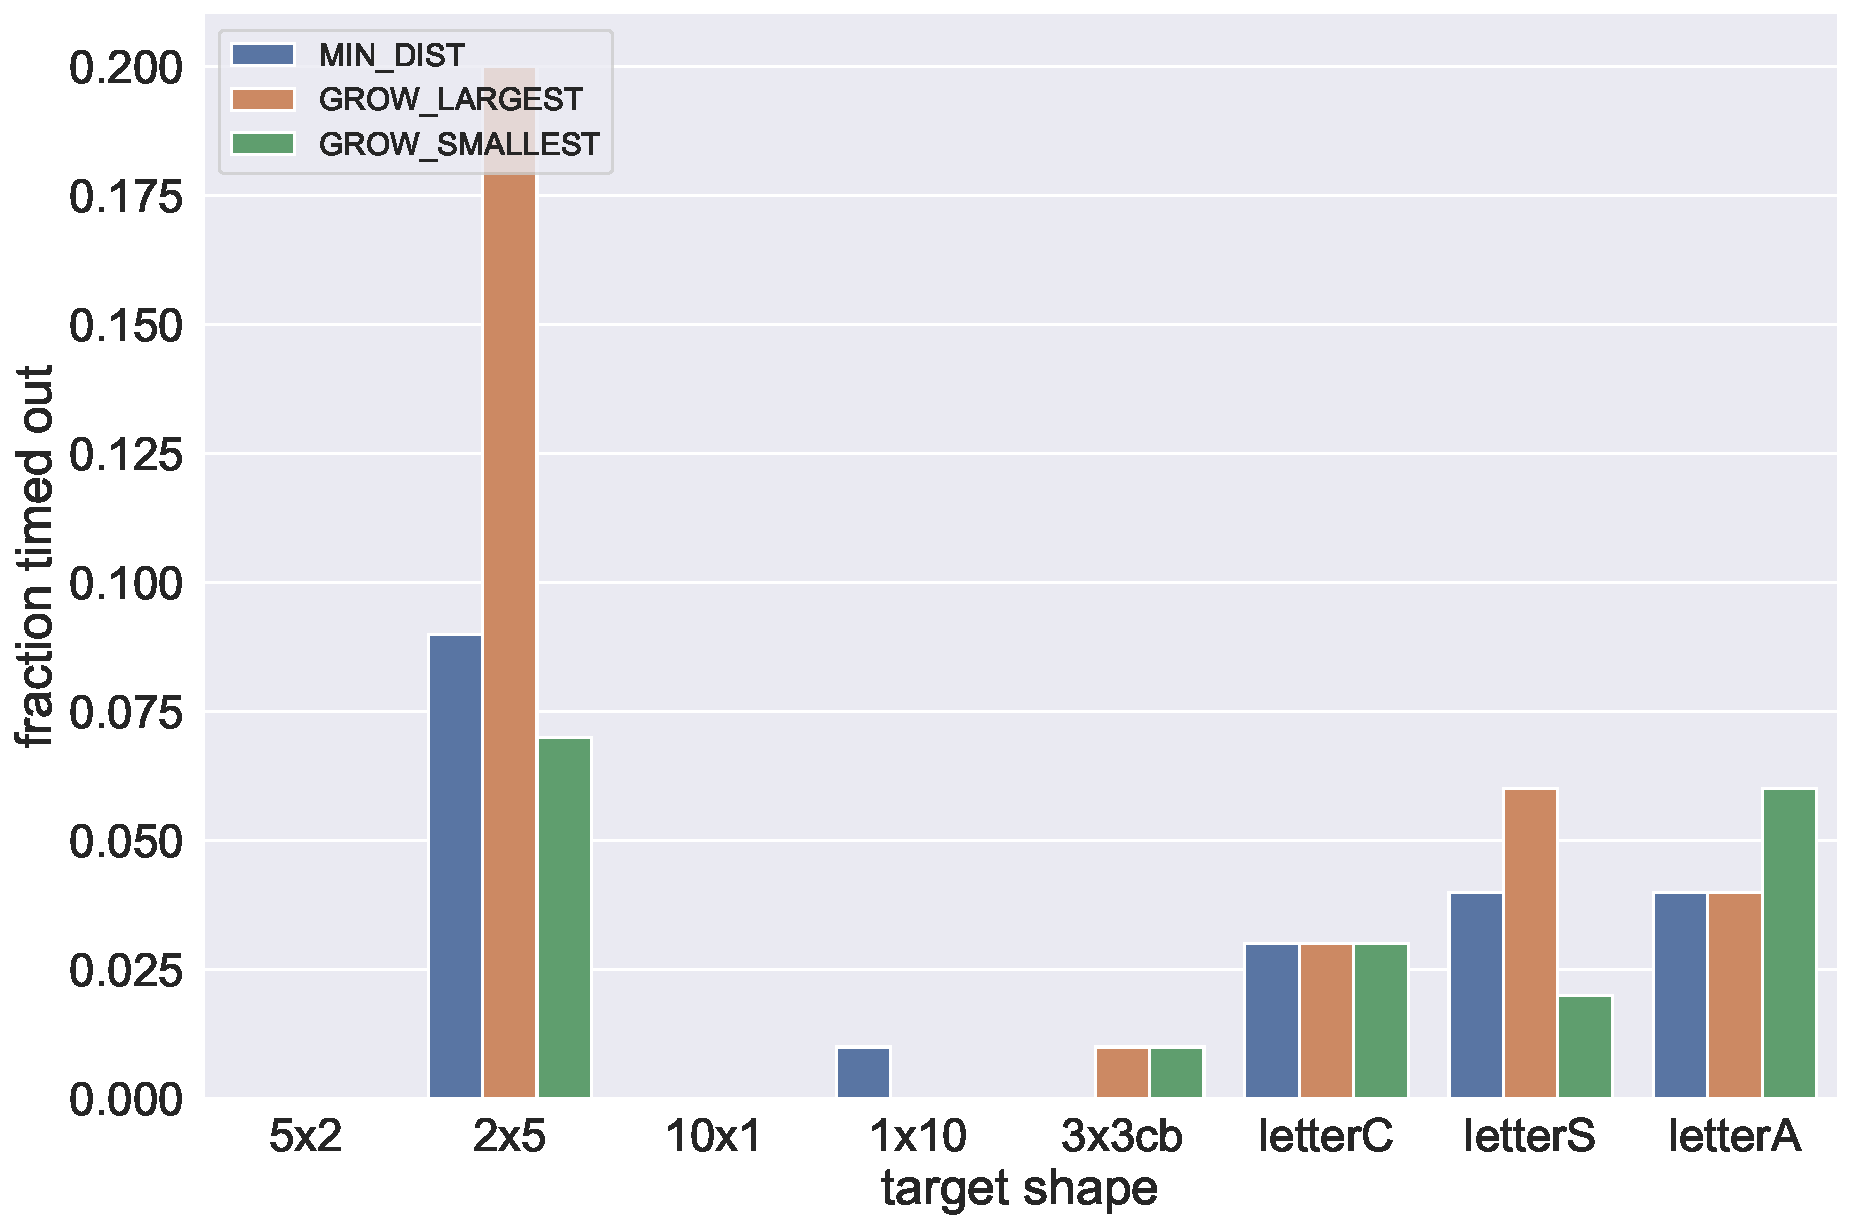
\includegraphics[width=0.9\textwidth]{figures/plots/AFTS_timeout.pdf}
		\caption{}
		\label{fig:AFTS_timeout}
	\end{subfigure}
	\caption[]{}
	\label{fig:AFTS_timestats}
\end{figure}




\section{Assembly for Workspace Size}

\begin{figure}
	\centering
	\begin{subfigure}[b]{\textwidth}
		\centering
		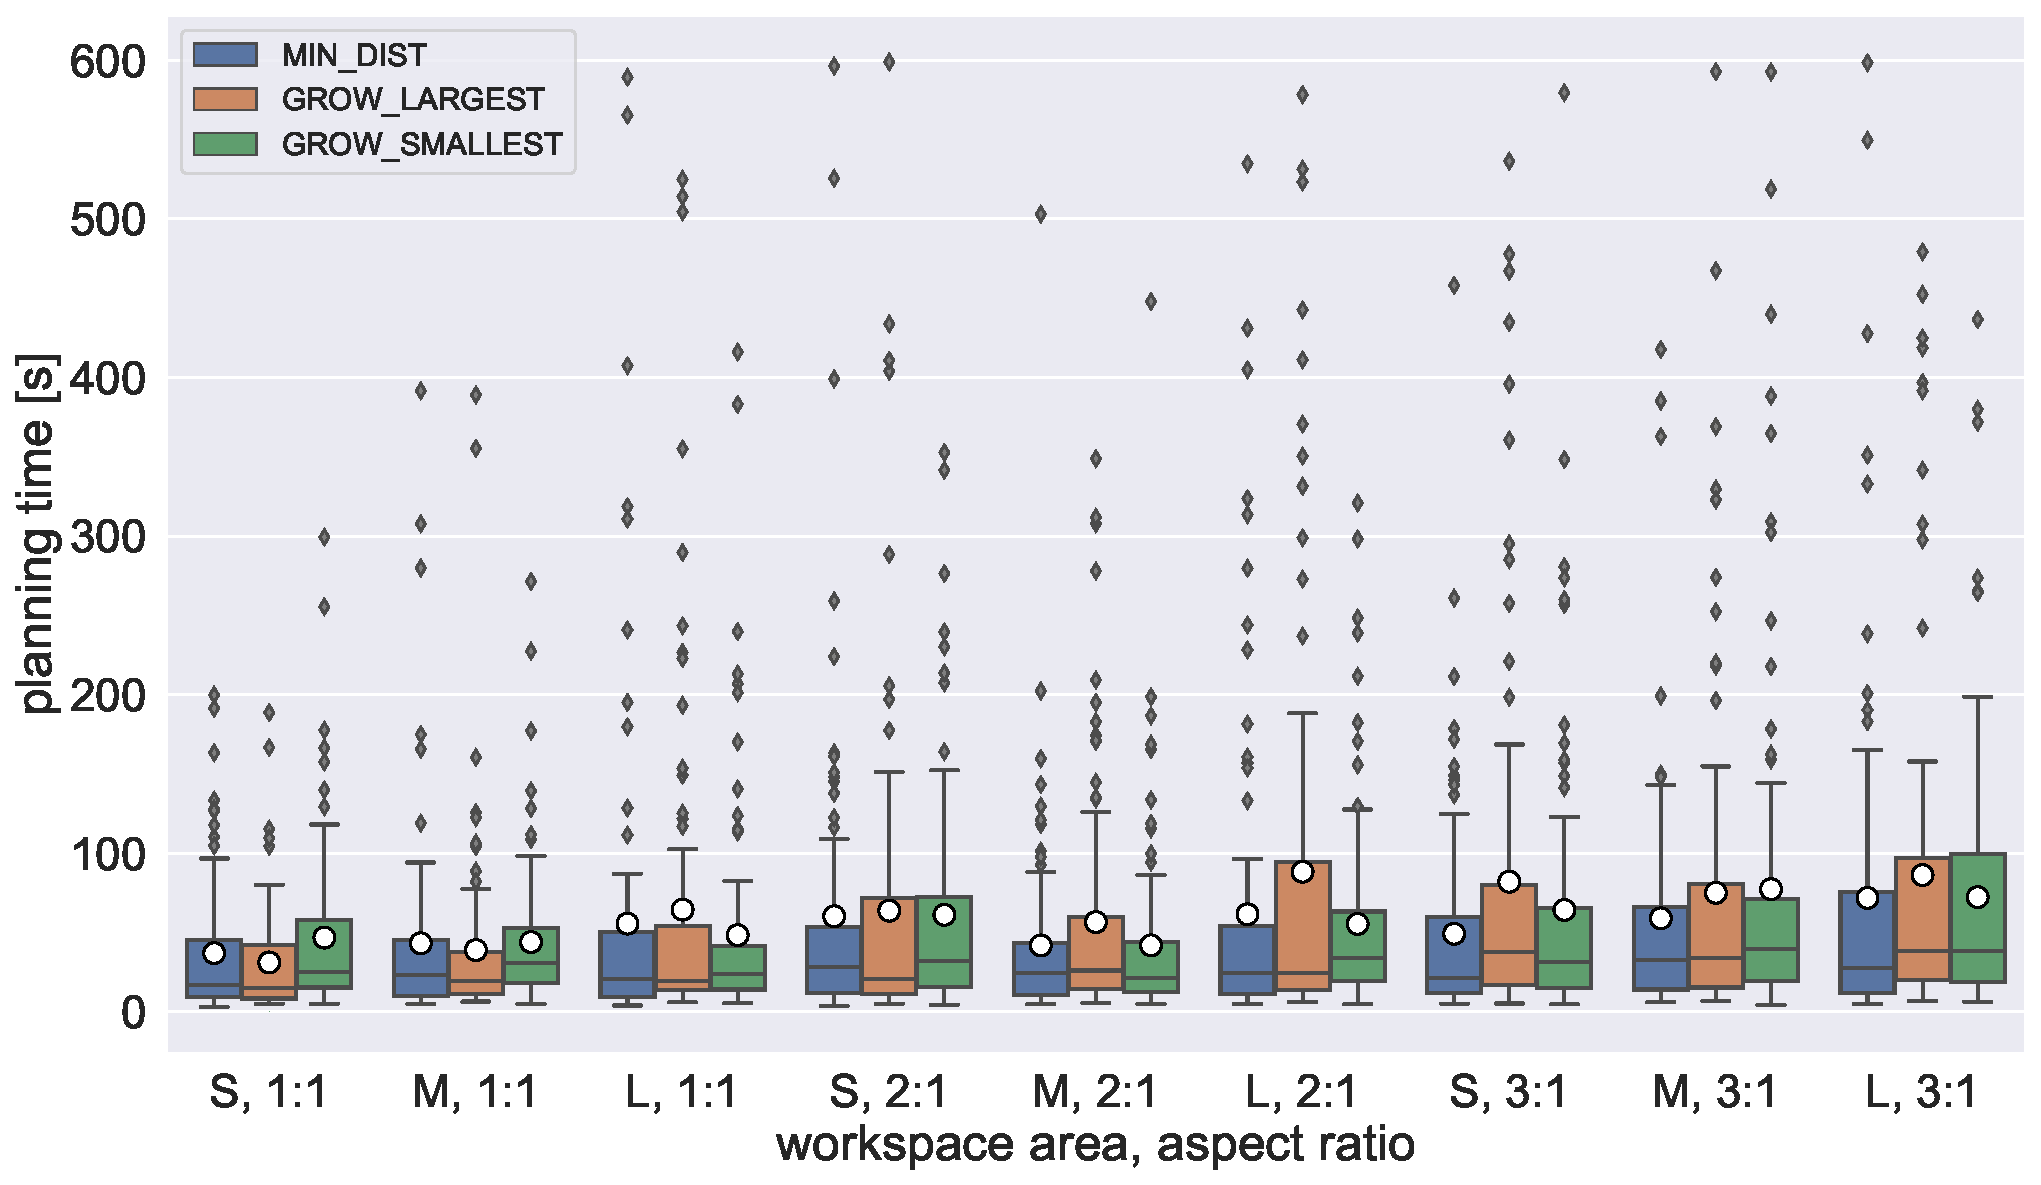
\includegraphics[width=0.9\textwidth]{figures/plots/AFBS_time.pdf}
		\caption{}
		\label{fig:AFBS_time}
	\end{subfigure}
	
	\begin{subfigure}[b]{\textwidth}
		\centering
		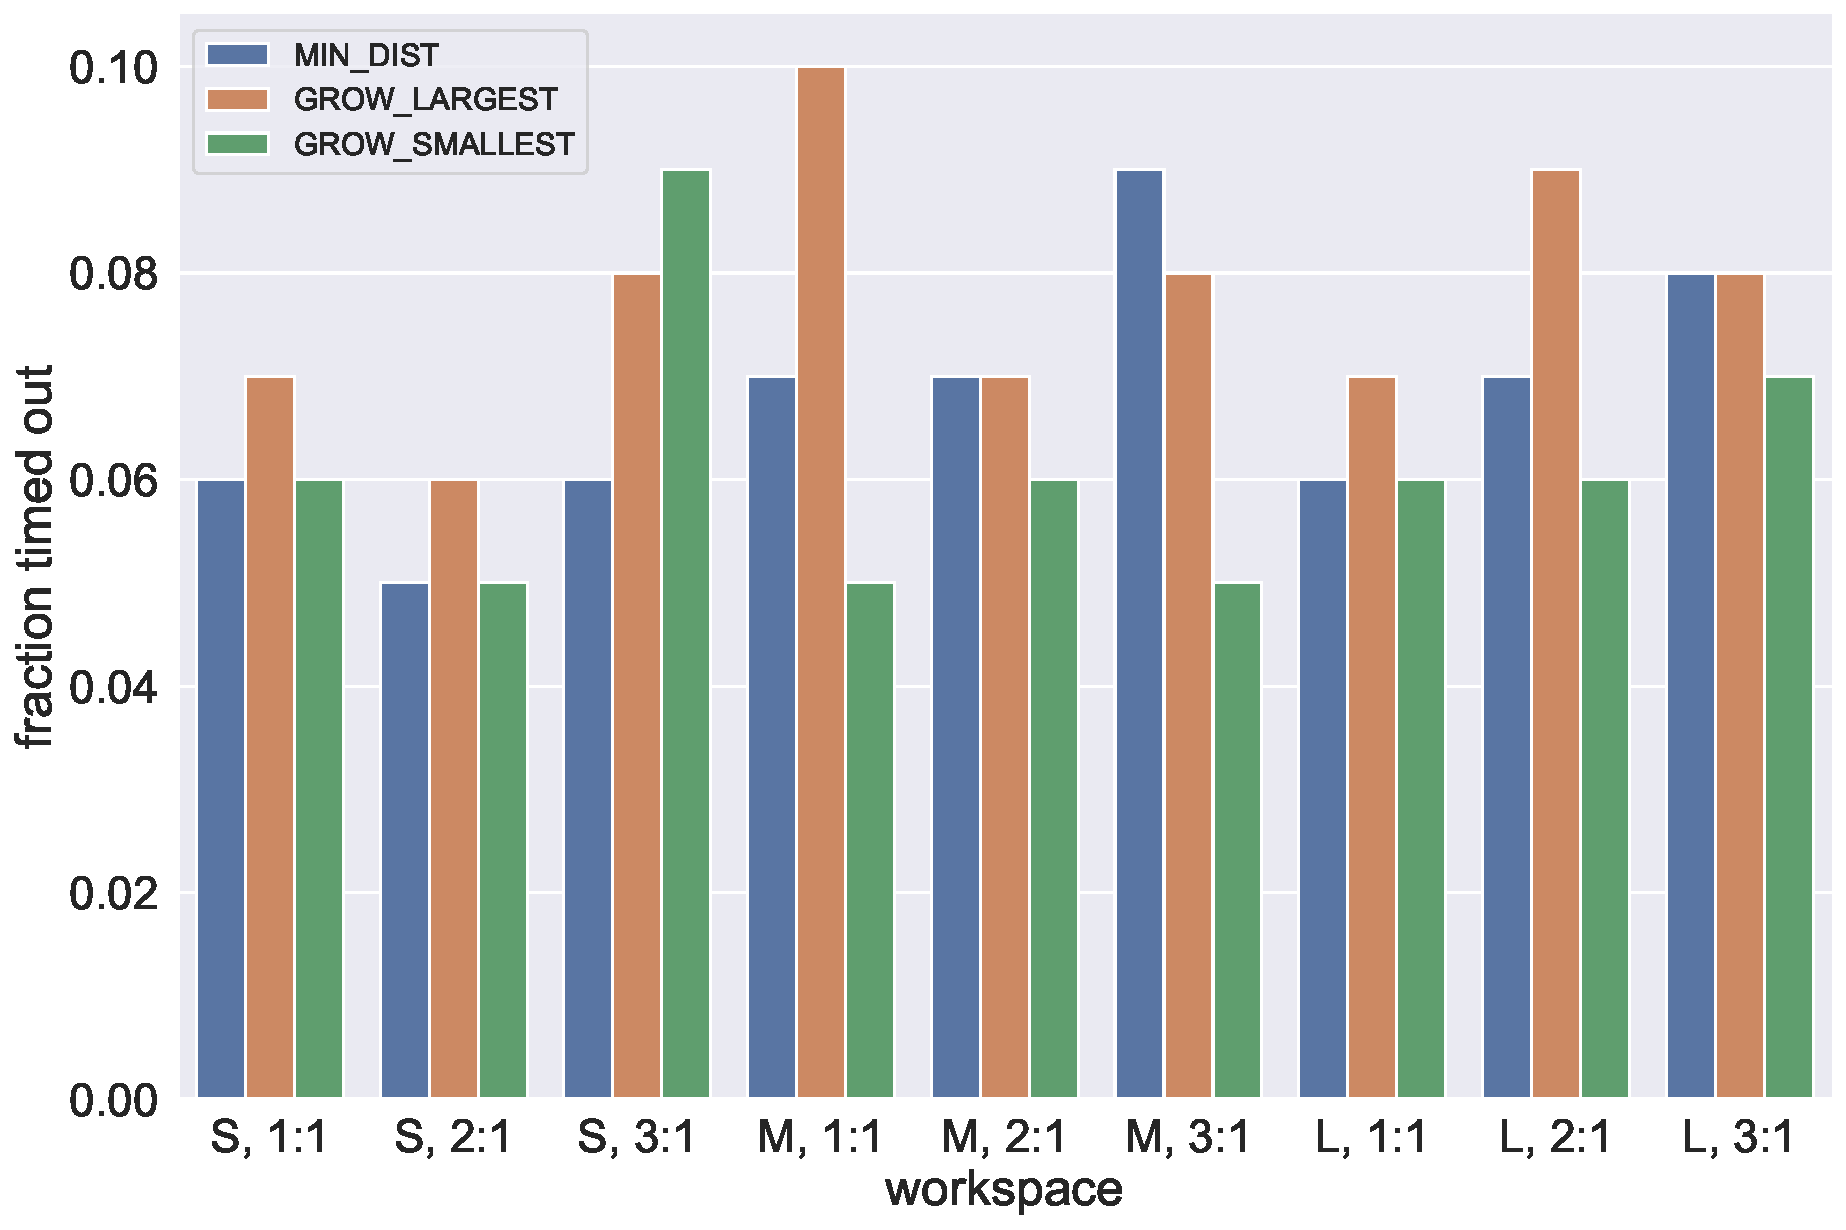
\includegraphics[width=0.9\textwidth]{figures/plots/AFBS_timeout.pdf}
		\caption{}
		\label{fig:AFBS_timeout}
	\end{subfigure}
	\caption[]{}
	\label{fig:AFBS_timestats}
\end{figure}

\begin{figure}
	\centering
	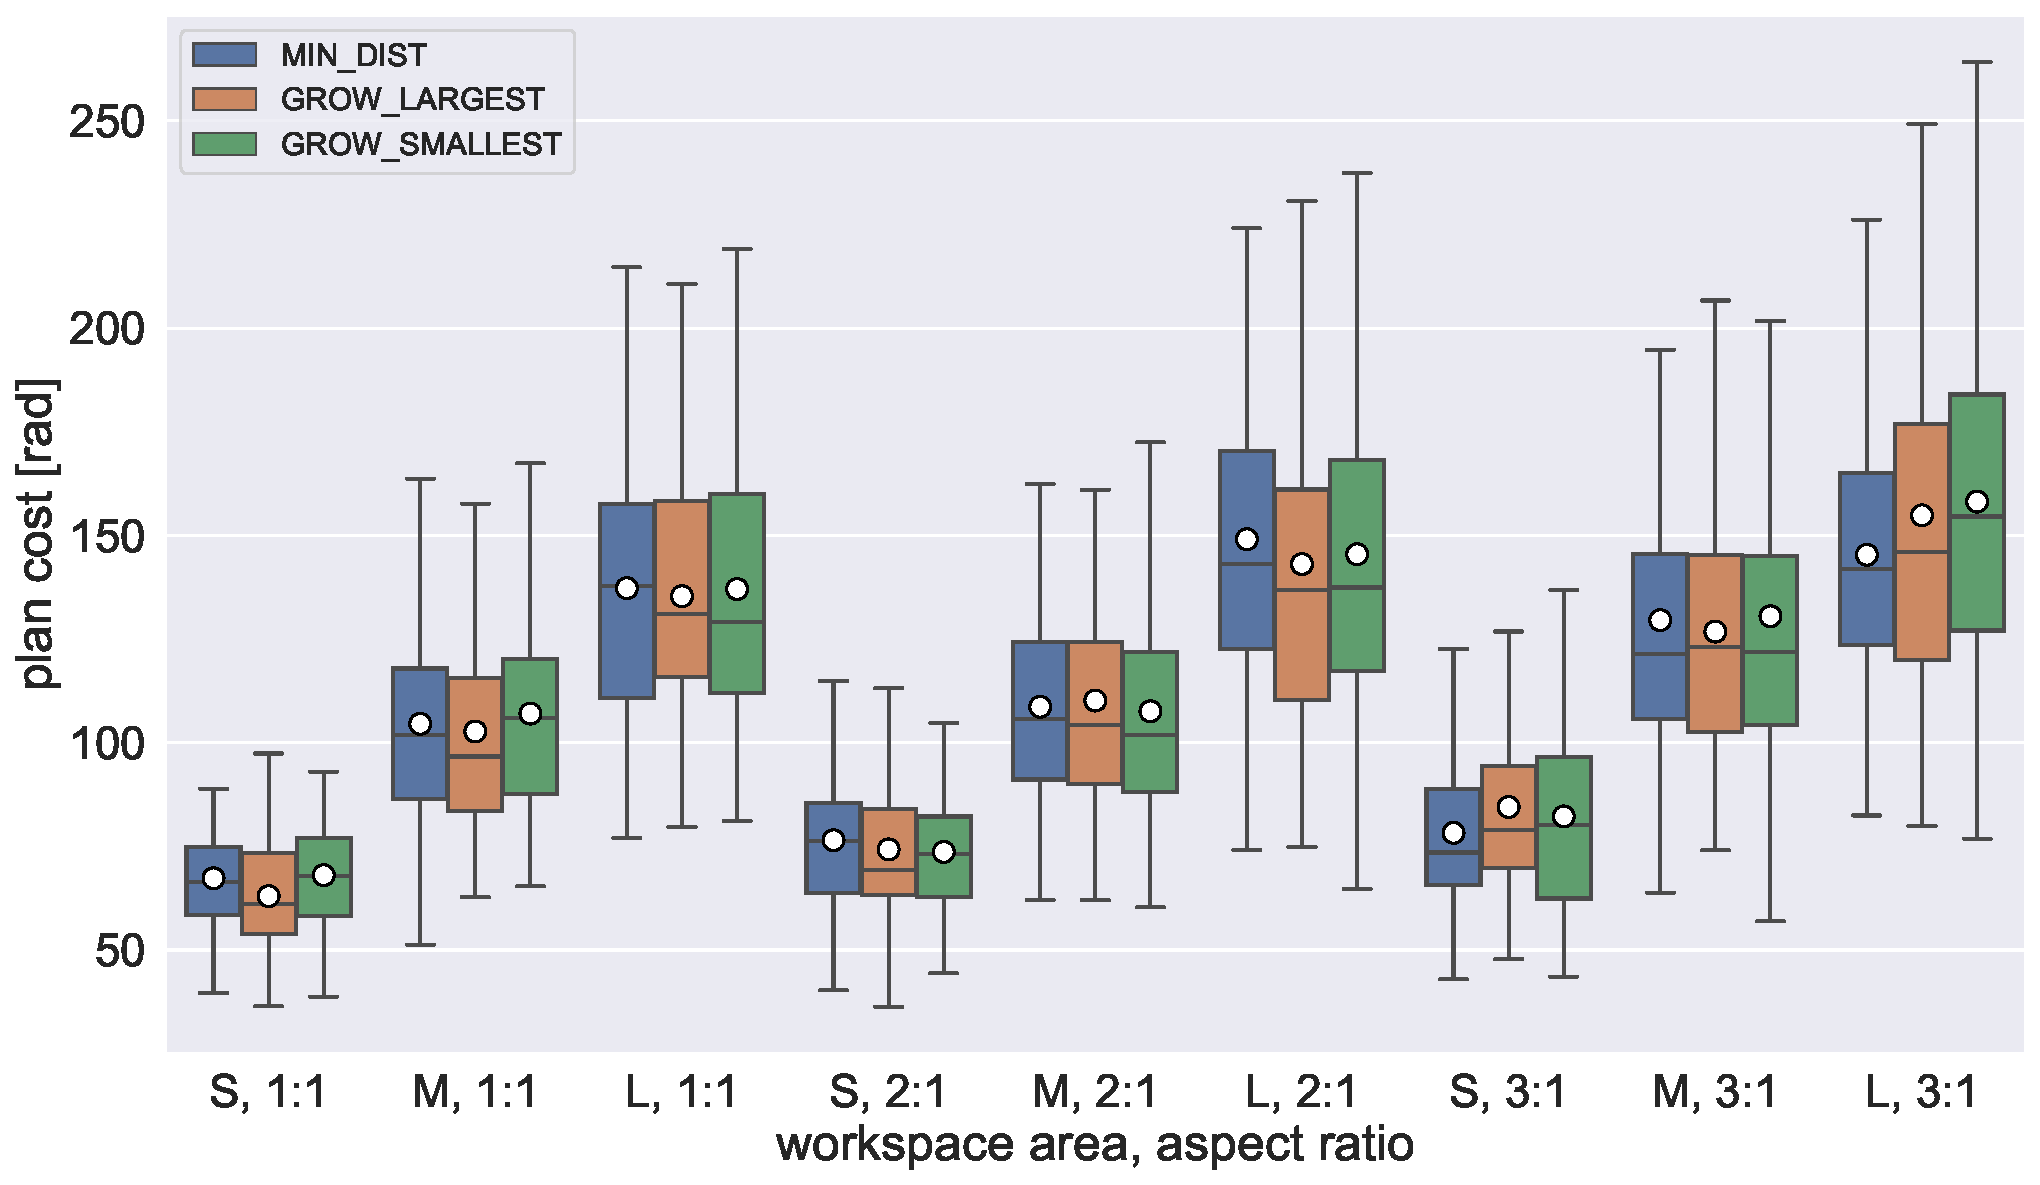
\includegraphics[width=0.9\textwidth]{figures/plots/AFBS_cost.pdf}
	\caption[]{}
	\label{fig:AFBS_cost}
\end{figure}



